\section{Definition of Hazards}
The dominant hazard in this experiment is the formation and combustion of a flammable gas
mixture.  The detector is operated in the avalanche regime, meaning that the detector voltage is near the breakdown voltage of the ionizing gas.  As a result, sparks are a common occurrence from the very nature of the detector and could serve as a possible ignition source.  Therefore, the chief safety concern related to the PGAC is preventing a combustible gas 
mixture from  forming.

%\subsection{Description}
\subsection{High Voltage}
The PGAC operates with an applied voltage difference up to 620\,V. The high-voltage power is supplied from standard HV supplies from the TRIUMF and EMMA equipment pools, including Bertan 1755P, Mesytech MHV-4, and Iseg NHQ 204M modules.  Connections to the detector chamber are made using standard HV cables and connectors. The exposed high voltage electrodes inside the chamber are not accessible without first venting and then dismantling the chamber.  Therefore, the use of high voltage is not considered a safety concern.  Furthermore, in accordance with TRIUMF Safety Note 5.11, voltages below 750\,V are defined as low voltages and do not require special consideration.
\subsection{Flammable Gas}
\label{flame}
The PGAC is filled with %12.6\,L of 
isobutane, which is gaseous at room temperature and highly-flammable.
Table~\ref{isobutane} summarizes the properties of isobutane.
The dominant hazard due to isobutane would be the formation and ignition of a flammable mixture of air and isobutane.
\begin{table}
%\begin{minipage}{\textwidth}  
\begin{center}
\begin{tabular}{p{0.45\columnwidth}|p{0.45\columnwidth}} 
%\begin{tabulary}{0.45\columnwidth}{R|L} 
\raggedleft Chemical equation&C$_4$H$_{10}$\\
\raggedleft IUPAC name&2-methylpropane\\
\raggedleft Commercial name&R-600a (refrigerant)\\
\raggedleft Molar mass&58.12\,g/mol\\
\raggedleft Specific gravity&2.07\\
\raggedleft {Lower flammable limit (LFL)}%\footnote{hello}
& {1.83\%}\\
\raggedleft Upper flammable limit (UFL)&8.43\%\\
%Flammable range in air (760\,Torr, 20$^\circ$\,C)&1.8--8.4\%\\
\raggedleft Stoichiometric concentration %(air)
&3.12\% \\
\raggedleft Peak-to-initial pressure ratio %P$_\textrm{f}$/P$_\textrm{i}$
&8.1--8.4:1\\%8.0
\raggedleft Auto ignition temperature% (air, 1\,bar)
&462$^\circ$\,C\\
\raggedleft Heat of combustion% (25$^\circ$\,C, 1\,bar)
&%45.8\,kJ/g
2,871\,kJ/mol% or  686.3\,kcal/mol or  49.40\,kJ/g
\\
%\raggedleft Paschen minimum (iBu)&420\,V, 4\,mbar-mm\\
%\raggedleft Paschen minimum (Air)&330\,V, 7.3\,mbar-mm\\
\raggedleft Flame speed (maximum)&0.37\,m/s\\
\raggedleft Adiabatic flame temperature&%2246?
2321\,K\\
\end{tabular}\\
%\begin{tabular}{r|l}
%  -&-\\
%\end{tabular}
\end{center}

\caption{ Physical properties of isobutane.  Isobutane is a chemical isomer of butane.  It is an alkane hydrocarbon, also called a paraffin hydrocarbon. %  Unless specified, 
All values are given at standard temperature and pressure in air.}
\label{isobutane}
%\footnotetext{hello}
%\end{minipage}
\end{table}

\subsubsection{Reaction}
The oxidation reaction of %combustion of air and
isobutane produces gaseous CO$_2$ and liquid water.  The chemical equation of the combustion of isobutane with oxygen is given below.
\begin{equation}
\textrm{C}_{4}\textrm{H}_{10} + 6.5 \textrm{O}_{2} %+ 26 \textrm{N}_{2}
\rightarrow 4 \textrm{CO}_{2} + 5 \textrm{H}_{2}\textrm{O} %+ 26 \textrm{N}_{2}
\label{reaction_eq}
\end{equation}
% C$_{4}$H$_{10}$ + 6.5 O$_{2}$ +26 N$_{2}$ $\rightarrow$ 4 CO$_{2}$ + 5 H$_{2}$O + 26 N$_{2}$
As indicated in Eq.~\ref{reaction_eq}, the stoichiometric (mole) ratio between isobutane and oxygen is 1:6.5.  In dry air at standard temperature and pressure, this corresponds to a volume concentration of 3.12\% isobutane or a mass concentration of 82.5\,mg/L.  Equivalently, a stoichiometric mixture of isobutane and air corresponds to an isobutane-to-air volume ratio of 1:31.0.  By definition, a stoichiometric concentration corresponds to an equivalence ratio, $\phi$, of 1.  Fuel-rich mixtures have a ratio $\phi>1$, fuel-lean mixtures have a ratio $\phi<1$.

Given an ignition source and a flammable mixture of isobutane and air, the resulting combustion will produce an explosive increase in pressure in the chamber.  In terms of this safety review, the key properties of isobutane combustion are its flammability limits and the maximum change in pressure due to an explosion.

\subsubsection{Flammability Limits}
The upper flammability limit (UFL) and the lower flammability limit (LFL) are the limiting fuel concentrations that can support flame propagation.  Outside of these concentration limits, an otherwise flammable gas is rendered non-flammable.  %For confined %stoichiometric combustion, 
The measured quantities associated with %the
combustion are dependent, in part, on the size and shape of the test chamber \cite{Takahashi_2003} and the decision criterion \cite{DeSmedt_1999} used in the measurements.  As a result, there is variation in the reported physical properties recorded in the literature.  Specifically, the flammability limits are empirical in nature and should not be regarded as intrinsic \cite{Zabetakis_1965}.
%Oxygen concentration
\paragraph{Atmospheric pressure}
There is a variety of data on the flammability limits of isobutane at and above atmospheric pressure reported in the literature.  The long-established values reported in Ref.~\cite{Jones_1947} and shown in Table~\ref{isobutane} give a flammability range of isobutane in air of 1.83--8.43\%.  The LFL corresponds to an equivalence ratio $\phi=0.59$ %, a mass concentration of 48.3\,mg/L,
and a fuel-to-air ratio of 1:53.6.  The UFL corresponds to an equivalence ratio of $\phi=2.7$ %, a mass concentration of 223\,mg/L
and a fuel-to-air ratio of 1:10.9.
A more recent study \cite{Kondo_2007} measured the flammability range of isobutane to be 1.68--7.8\%.  The variation in the measured flammability limits is on the order of 10\%, however, that translates to less than 1\% difference in volume concentration.

\paragraph{Subatmospheric pressure}
%\subsubsection{Low pressure}
%It should also be noted, as the pressure of a system reduces, eventually a point is reached where flammability is not supported.  
Since the PGAC operates at 3--6\,Torr, the flammability characteristics of isobutane at low pressure are relevant.  Little data exists on sub-atmospheric combustion, however, it is widely reported that, in general, at pressures below 45\,Torr flame propagation stops and combustion is impossible \cite{hazard}. % Edwards
The study reported in Ref.~\cite{Scott_1952} is unique in having measured the flammability limits of a number of hydrocarbons, both as a function of concentration and pressure. Fig.~\ref{lowpres} shows the results for isobutane.  Below 40\,Torr isobutane is non-flammable.

A recent pair of measurements also studied the upper \cite{Le_2012} and lower \cite{Le_2013} flammability limits at subatmospheric pressure.  Their measurements are consistent with Ref.~\cite{Scott_1952}, however, their measurements stopped at 76\,Torr and did not investigate the lowest pressure that supports combustion. 

\begin{figure}[t]%
\centering  
%\includegraphics[width=\columnwidth,keepaspectratio]{Scott_1952-fig7}%
%\includegraphics[height=3in,keepaspectratio]{Jones_1947-fig1}
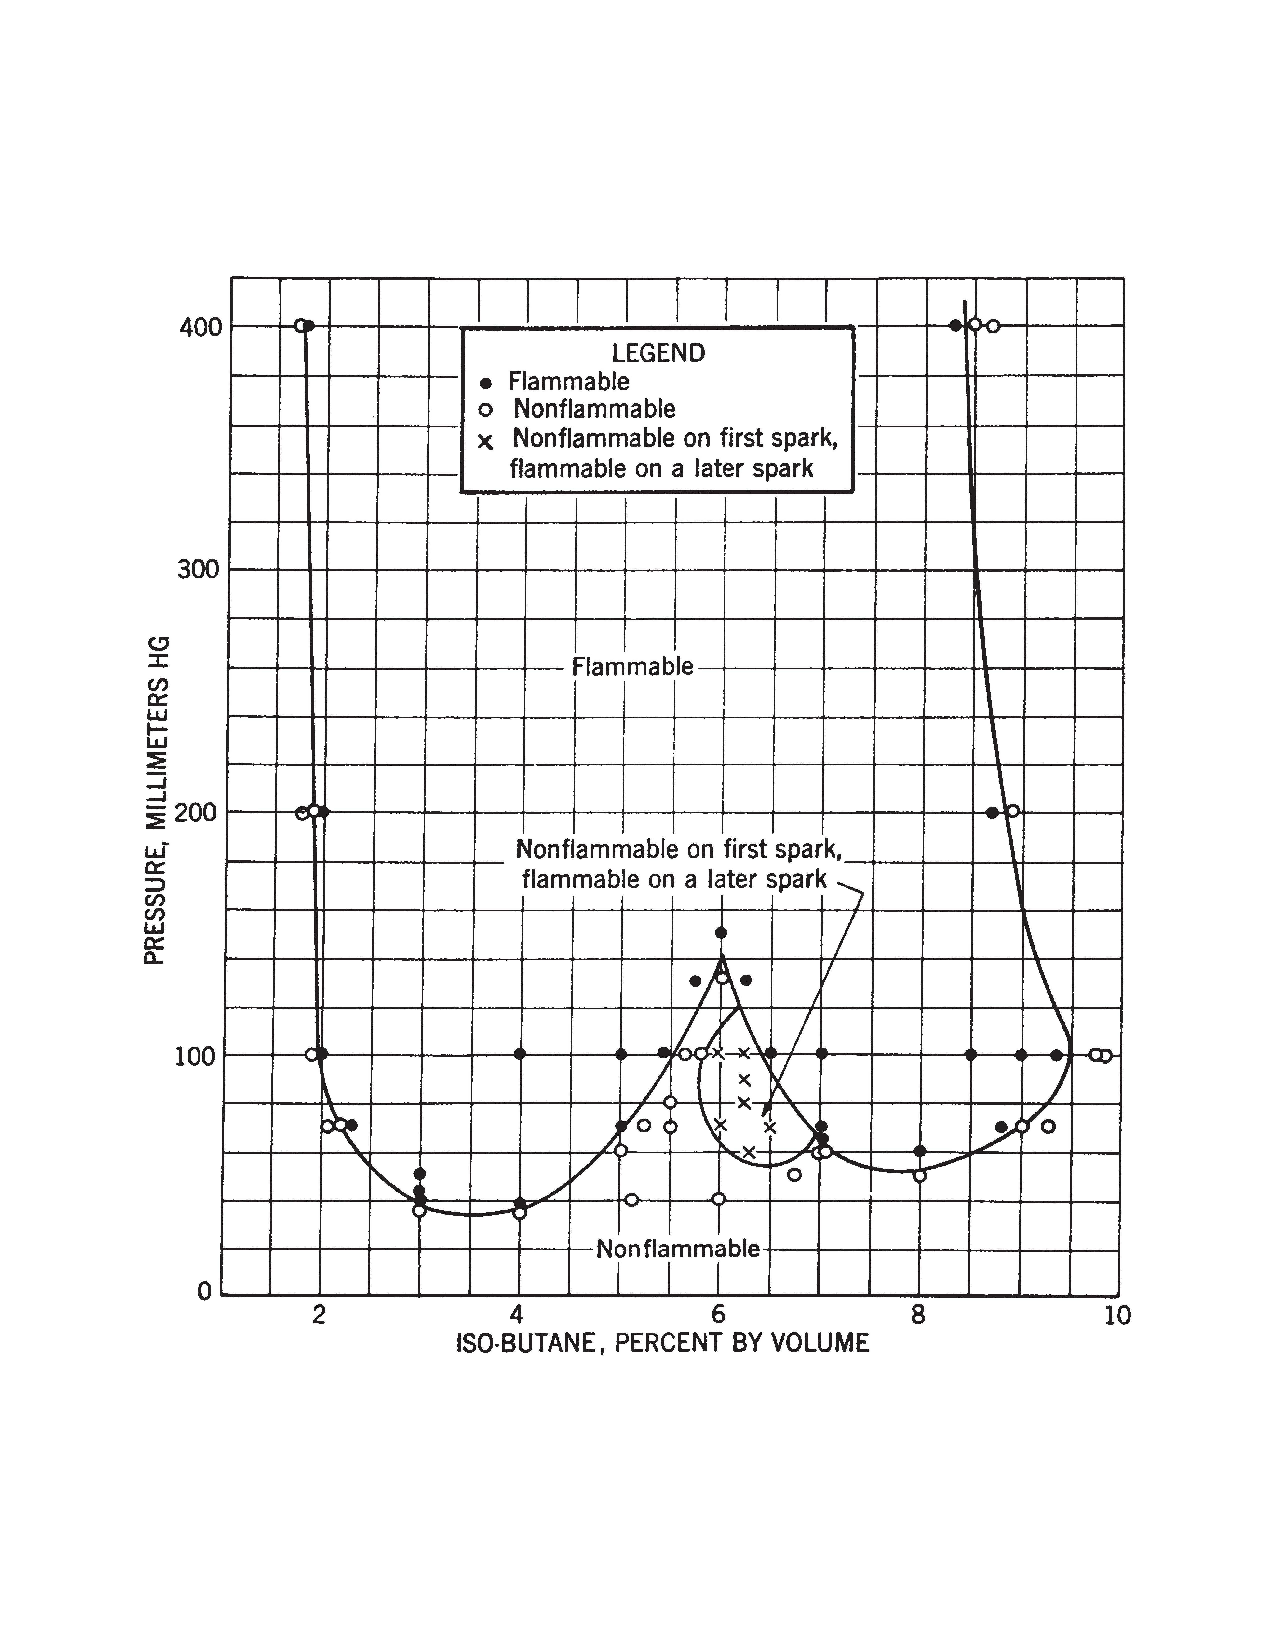
\includegraphics[width=\textwidth,height=0.5\textheight,keepaspectratio]{Scott_1952-fig7c}%
\caption{Flammability of isobutane at subatmospheric pressure.
%(Left) Figure from Ref.~\cite[Fig.~1]{Jones_1947}. (Right) %Flammability at subatmosphereic pressure.
Below 140\,Torr, the flammability limit becomes double-valued.  Below 40\,Torr, no concentration of isobutane is flammable.  Figure taken from Ref.~\cite[Fig.~7]{Scott_1952}}%
\label{lowpres}%
\end{figure}

\subsubsection{Pressure Change}
\paragraph{Isobutane} The possible increase in pressure due to combustion is the main hazard arising from the use of isobutane.  The rate of pressure increase and magnitude of the peak-to-initial pressure ratio is a minimum at the flammability limits and at a maximum near the stoichiometric ratio \cite{Zabetakis_1965}.
At standard temperature and pressure, the maximum flame propagation speed during the combustion of isobutane is about 36.7\,cm/s \cite{Davis_1998}.  This flame speed is well below the speed of sound (34,029\,cm/s), making the explosion a deflagration, as opposed to a detonation.  The peak flame speed occurs at an equivalence ratio of $\phi=1.1$.

A typical value of the peak-to-initial pressure ratio for the confined deflagration of a hydrocarbon is 8:1 \cite{Zabetakis_1965}.  This value can be calculated using the ideal gas law by taking the ratio of the adiabatic flame temperature of the combustion to the initial ambient temperature.  A number of studies have also determined this value empirically.
A somewhat dubious report published in Ref.~\cite{Zgliczynski_1994} claims a maximum peak-to-initial pressure ratio of 7.75 occurring at isobutane concentration of 3.5\%.  This concentration corresponds to an equivalence ratio of $\phi=1.12$ and a fuel-to-air ratio of 1:27.6.

\paragraph{$n$-butane} Ref.~\cite{Razus_2007} presents an extensive measurements of the pressure evolution of $n$-butane and air mixtures over a range of initial pressures and concentrations using different test chambers.  The maximum peak-to-initial pressure ratio and the maximum rate of pressure increase occur at a volume concentrations of 3.63\%.  This corresponds to an equivalence ratio of $\phi=$1.16, slightly above the stoichiometric ratio, and a fuel-to-air ratio of 1:26.5.  The maximum explosive pressure ratio measured was 9.34:1 for a spherical chamber and 9.01 for a cylindrical chamber.

Note that data for $n$-butane may be substituted  for isobutane in some cases.  For example, isobutane and $n$-butane, being chemical isomers, have the same molecular weight, specific gravity, and stoichiometric concentrations.
The flammability limits of the alkane hydrocarbons vary as a function of their molecular weight \cite{Zabetakis_1965}.  Consequently, studies of the flammability limits of $n$-butane are applicable to isobutane.  Additionally, Ref.~\cite{Davis_1998} shows that $n$-butane and isobutane have maximum flame speed at the same equivalence ratio.  The flame speed of $n$-butane reported in Ref.~\cite{Davis_1998} is about 40.8\,cm/s, or 111\% of the flame speed of isobutane.  Given that flame speed and explosion pressure are intimately related, the peak-to-initial pressure ratio of isobutane should be approximately 89.0\% of that reported for $n$-butane.  This assumption corresponds to an explosive pressure ratio for isobutane of %8.1--
8.4:1.

\paragraph{Shape dependence} As mentioned, the pressure evolution during an explosion depends on the shape of the chamber.  The time to peak pressure is proportional to the cube-root of the volume of the chamber \cite{Zabetakis_1965}. Based on the 12.6\,L volume of the PGAC box, the peak pressure should take approximately 57.3\,ms to develop.  However, this approximation assumes either spherical or cylindrical symmetry.  The parallelpiped configuration of the PGAC box may inhibit the production of pressure waves and reduce the maximum explosive pressure.


\subsection{Leak Scenarios}
%Potential sources of a leak are as follows.
\subsubsection{Worst-case scenario}
The worst-case would be the ignition of a near-stoichiometric mixture ($\phi=1.16$) of air and isobutane at atmospheric pressure  inside the confined volume  of the PGAC box. %, with the diagnostic box at atmospheric pressure.
This scenario requires a leak into the chamber to introduce air in a ratio of 26.5:1 to isobutane, resulting in a 3.63\% volume concentration of isobutane.  This concentration would produce a maximum explosive pressure of 6,380\,Torr (8.4\,atm) %8.51\,bar
inside the volume of the PGAC box.
%(30\,mbar iBu + 983\,mbar air),(1.5\,L)

If this scenario did occur, the resulting pressure increase would cause %at least one of the two 
the Mylar window to burst 
%at 24\,Torr differential pressure 
and vent the gasses into the 50\,L volume of the $0^{\circ}$ scattering chamber. The initial pressure in the scattering chamber would necessarily have been 760\,Torr %1.01\,bar
since the PGAC window can only support 57\,Torr of %limited
 differential pressure. The resulting maximum pressure in the combined volume would be
 1,890\,Torr (2.49\,atm or 1.49\,atm gauge pressure).
 %2.52\,bar (1.51\,bar gauge pressure).
 It should be noted that the Mylar window would break before the peak explosive pressure in the PGAC box could be reached.  The resulting dilution of the gas mixture would rapidly bring the concentration of isobutane below the flammability limit and quench flame propagation.

In reality, this scenario would be extremely difficult to achieve. The PID controller turns off the isobutane supply at pressures greater than its setpoint, which has a maximum value of of 10\,Torr.  Additional interlocks shut off the isobutane flow and the HV power if the diagnostic box pressure exceeds $\textrm{P}_\textrm{max}=7\times10^{-5}$\,Torr.  The required simultaneous, rapid influx of air filling the independent volumes of the PGAC box and the scattering chamber would almost certainly rupture the PGAC window and trip pressure interlocks that turn off the HV.  Even if HV interlocks failed and the bias was left constant, the increasing gas pressure would rapidly raise the breakdown voltage above the bias voltage, removing the source of ignition. %\cite{Heylen_1956}

\subsubsection{Low-pressure scenarios}
\label{low_pres}
\paragraph{UFL} A less contrived version of the worst-case scenario, i.e., one that does not require the simultaneous failure of multiple interlocks, would be an % massive
air leak into the volume of the PGAC box which is initially filled with 6\,Torr of isobutane.  With such a leak, %an air leak into isobutane, 
a flammable mixture would first form at the UFL when the concentration of isobutane is reduced to 8.43\%.  The fuel-to-air ratio of this mixture is 1:10.9.  The flow rate of isobutane into the detector is typically set at 60\,cc/min.
%0.10 Standard Liters per Minute (SLPM). 
 Assuming an air leak is already present when the detector gas flow was set, this would require a minimum air leak of 651\,cc/min
% 1.09\,SLPM
to form a combustible mixture.  

At the UFL, the total initial pressure in the PGAC box would be 71.2\,Torr. %142
  It is plausible %, however unlikely,
that the Mylar window could tolerate a pressure differential this high long enough to produce a flammable mixture.  If the flammable mixture was ignited, the resulting explosion would burst the Mylar window.  Since the explosion would be occurring at the limit of flammability, the peak-to-initial explosion pressure would be less than the maximum of 8.4:1.  Extrapolating from measurements with butane \cite{Razus_2007} and comparing to data for hydrogen \cite{Dahoe_2005}, at an equivalence ratio of $\phi=2.7$ the peak-to-initial explosion pressure ratio would be about 6.4:1.  Such an explosion would produce a maximum pressure in the combined  volume of the PGAC box and the scattering chamber of 91.7\,Torr. %183
% If the scattering chamber was also at an initial pressure of 71.2\,Torr, the final pressure of the system would be 149\,Torr.

\paragraph{Stoichiometric mix} An air leak leading to a stoichiometric gas mixture would have a higher explosion pressure.  However, in order to reach the stoichiometric fuel-to-air ratio of 1:31.0, a sustained air leak of 
1,860\,cc/min
%3.10\,SLPM
 would be required.  At the stoichiometric ratio, the pressure in the PGAC box would be 
 192\,Torr. %384
   This pressure is %near the upper limited of the estimated 
 so far above the
 burst pressure of the Mylar window that %, therefore
 it is unlikely that this gas mixture could be contained in the volume of the PGAC box.  Once dispersed into the 50\,L volume of the $0^\circ$ scattering chamber, the pressure of the gas mixture would be reduced to 38.7\,Torr %77\,Torr.  The resulting explosion would raise the pressure in the combined volume of the PGAC box and the scattering chamber to 495\,Torr.
 and ignition would be impossible.
 %Similarly, if the PGAC was operated at pressures above 6\,Torr, flammable gas mixtures could only be formed after the Mylar window has burst.

\paragraph {LFL}A scenario in which the PGAC box is accidentally vented would produce an even higher flow rate of air into the chamber.  However, such a leak  could only produce a gas mixture at or near the stoichiometric ratio for the reasons just discussed.  Namely, the Mylar window would break before a fuel-lean air mixture could be achieved.  Starting with an initial pressure of 6\,Torr of isobutane, % in the PGAC chamber, 
the LFL would be reached when the pressure in the PGAC box reached 328\,Torr. %656
 If this mixture were ignited, the resulting pressure in the combined volume of the PGAC box and the scattering chamber would be 422\,Torr. %845
   The analogous scenario resulting from the accidental venting of the scattering chamber could not produce a flammable mixture.  The pressure in the 50\,L scattering chamber required to burst the Mylar window would produce a gas mixture far below the LFL.

\subsubsection{Bellows damage }
A rupture in the beam line or the pumping system could cause an air leak into the chamber.  The most delicate component of these systems is the upstream bellows.  However, damage to the bellows is highly unlikely because the stable support of the chamber prevents any
mechanical stresses being applied to the bellows.

\subsubsection{Valve failure }
The only valves that ultimately open to air are in the roughing line and the venting line.  This would
require the simultaneous failure of 2--3 valves as show in Eq.~\ref{valve_fail}.  It should be noted that all of these combinations include at least one automatic valve which closes in the event of a power failure. % An air leak would require failure of the fail-safe.
In addition, if the pump valve was part of the failure, the roughing pump itself would also have to fail.  The coincidental failures required for a leak in the roughing line or the venting line is unlikely.

\begin{equation}
[\texttt{HEBTBV19} \lor (\texttt{HEBTRV19} \land \texttt{HEBTVV19A})] \land  (\texttt{HEBTTPV19} \lor \texttt{HEBTRV19})
\label{valve_fail}
\end{equation}

\subsubsection{Gas line damage (low pressure)}
If a leak develops the sub-atmospheric portion of the plumbing, the gas handling system will automatically decrease the detector gas flow rate to maintain the pressure. In this case, a far smaller leak would be needed to create a flammable mixture compared to a leak in the chamber.  With a total gas flow rate of 60\,cc/min,
%0.10\,SLPM,
an air leak of a 55\,cc/min
% 0.09\,SLPM
would be needed to create a combustible ratio mixture.  This is still a larger leak than one would expect from the Swagelok gas fittings used on the outside
of the chamber. Additionally, the flow rate of isobutane would visibly drop by 92\% from %0.10\,SLPM to 0.01\,SLPM,
60\,cc/min to 5.0\,cc/min,
which would trigger interlocks as detailed in \S~\ref{interlocks}.  It should be noted that at an operating pressure of 6\,Torr, this mixture would still not be flammable.

All sections of gas tubing which might be at sub-atmospheric pressure will be robust against
breakage. In particular, the tubing between \texttt{FC1} and the PGAC box; between the PGAC box, the scattering chamber, and valve
\texttt{VB4}; and between the gas supply panel and \texttt{VA1} should all be copper or stainless steel piping.
When possible, the roughing lines and will be located underneath the support structure which will act to protect them from external influences. %Similarly, the window bypass lines will be routed underneath the chamber.
Hence, damage to the low-pressure gas lines is unlikely.

\subsubsection{Gas line damage (high pressure)}
Leaks of isobutane from the above-atmospheric pressure portion of the plumbing into the surrounding air are not considered a significant hazard.  The stainless steel and copper plumbing lines used for the gas supply and exhaust are leaked-checked.  In the event of a complete line rupture, the maximum possible isobutane flow rate into the hall is only 250\,cc/min.

The air in the ISAC-II hall is replaced with fresh air every 11\,minutes (up to 110 minutes, depending on the recycled air ratio).
Tests under similar conditions have shown that a continuous 400\,cc/min isobutane leak would result in a flammable volume of less than 2\,L extending less than 30\,cm from the source of the leak   \cite{Openshaw_2006}. Additionally, a flammable gas sensor will be installed near the experimental area to detected any gas
leaks out into the ISAC-II hall.  An air leak into a sub-atmospheric volume containing isobutane and an ignition source would present a more significant hazard.

\subsubsection{Power failure} In the event of a power failure, all valves close and HV power supplies in the chamber latch off. The
scroll pump on the gas line is equipped with a valve that will default to closed so the chamber will
not vent to air. Thus, loss of power is not considered a potential hazard.